\documentclass[a4paper,11pt]{article}
\usepackage[utf8]{inputenc}
\usepackage[T1]{fontenc}
\usepackage{lmodern}
\usepackage{color}
\definecolor{darkblue}{rgb}{0.0, 0.0, 0.55}
\usepackage{setspace}
\usepackage[left=2.5cm, right=2.5cm, top=2.5cm, bottom=2.5cm]{geometry}
\usepackage[backref,pagebackref]{hyperref}
\usepackage[authoryear]{natbib}
\usepackage{graphicx}
\usepackage{lscape}
\usepackage{amsmath}
\usepackage{indentfirst}
\usepackage{tikz}
\usetikzlibrary{positioning}
\newdimen\nodeDist
\nodeDist=35mm
\usepackage{forest}
\usepackage[english]{babel}
\usepackage{babelbib} 
\newcommand\bookepigraph[4]{
\vspace{1em}\hfill{}\begin{minipage}{#1}{\begin{spacing}{0.9}
\small\noindent\textit{#2}\end{spacing}
\vspace{2em}
\hfill{}{#3}\small\\
\vspace{-2em}\begin{flushright}{#4}\end{flushright}}\vspace{1em}
\end{minipage}}
\usepackage{tikz-qtree}
\usepackage{qtree}
\usepackage{mathtools}
\usetikzlibrary{positioning}
\exhyphenpenalty=1000
\hyphenpenalty=1000
\widowpenalty=1000
\clubpenalty=1000

\renewcommand*{\backref}[1]{}
\renewcommand*{\backrefalt}[4]{%
    \ifcase #1 (N\~{a}o citado.)%
    \or        Cited on page~#2.%
    \else      Cited on pages~#2.%
    \fi}
\renewcommand{\backreftwosep}{ and~} 
\renewcommand{\backreflastsep}{ and~}

\hypersetup{pdftitle={Intelligent Policing and Homicide Prevention: Using the Synthetic Control Method to Estimate the Effect of Policy Implementation},pdfauthor={Danilo Freire, Rodolpho Barnabel},pdfsubject={},pdfkeywords={Brazil, urban violence, crime prevention, synthetic control},linkcolor=darkblue, citecolor=darkblue, urlcolor=darkblue, breaklinks=true, colorlinks=true}

\title{Intelligent Policing and Homicide Prevention:\\ Using the Synthetic Control Method to Estimate\\ the Effect of Policy Implementation\thanks{The authors are indebted to Andr\'{e} Amaro, Gustavo Ara\'{u}jo, F\'{a}bio Barros, Carlos Cinelli, Guilherme Duarte, Gabriela Ferreira, Rafael Magalh\~{a}es, Fernando Mour\'{o}n, Am\^{a}ncio Oliveira, Fl\'{a}vio Pinheiro, and David Skarbek for their helpful comments and suggestions. The usual disclaimer applies. All data, code, and \LaTeX \hspace{.001cm} files required to replicate this study are available at the following web address: \href{https://github.com/danilofreire/replication-files/tree/master/2015/intelligent-policing}{https://github.com/danilofreire/replication-files/tree/master/2015/intelligent-policing}.}}

\author{
Danilo Freire\thanks{Department of Political Economy, King's College London. Website: \href{http://danilofreire.com}{http://danilofreire.com}. Email address: \href{mailto:danilofreire@gmail.com}{danilofreire@gmail.com}. Corresponding author.}
\and Rodolpho Bernabel\thanks{Department of Politics, New York University. Website: \href{http://www.rodolphobernabel.com}{http://www.rodolphobernabel.com}. Email address: \href{mailto:rodolpho.bernabel@nyu.edu}{rodolpho.bernabel@nyu.edu}.}
} 

\date{\today\\
\vspace{2cm}
Preliminary Draft --- Comments Welcome\\
\vspace{.25cm}
Please do not cite or circulate without permission of the authors
}

\begin{document}

\maketitle

\begin{abstract}

\onehalfspacing

Although Brazil remains severely affected by civil violence, the state of S\~{a}o Paulo has made significant inroads in fighting criminality. In the last decade, S\~{a}o Paulo has witnessed a 70\% decline in homicide rates, a result that policy-makers attribute to a series of crime-reducing measures implemented by the state government. While recent academic studies seem to confirm this downward trend, no estimation of the impact of state policies on homicide rates currently exists. In this article, we fill this gap by employing the Synthetic Control Method to compare these measures against an artificial S\~{a}o Paulo. The results indicate a large drop in homicide rates in actual S\~{a}o Paulo when contrasted with our synthetic counterfactual, with about 20,000 lives saved during the period. The theoretical usefulness of the Synthetic Control Method for public policy analysis and the practical implications of the security measures taken by the S\~{a}o Paulo state government are also discussed.

\vspace{.5cm}
\noindent
\textsc{Keywords}: Brazil, urban violence, crime prevention, synthetic control
\end{abstract}

\newpage

\section{Introduction}

\doublespacing

Brazil has long been ravaged by an undeclared civil war. According to the Citizen Council on Public Security and Criminal Justice, a Mexican think-tank, no less than 19 of the 50 most violent cities in the world are located in Brazil \citep{mexico2014}.\footnote{The study disregards war zones and cities with unavailable data.} The 2014 Violence Map survey shows that 56,337 people were murdered in Brazil in 2012 alone \citep{mapa2014}, the highest incidence of intentional homicides on the planet \citep{unodc2013}. Paradoxically, the sharp rise in lethal violence has occurred during Brazil's longest period of political openness \citep{ahnen2003, pinheiro2000, pinheiro2001}. Over the past three decades, murder rates have increased by 148\%, jumping from 11.7 homicides per 100,000 people in 1980 to roughly 29 per 100,000 in 2012 \citep{mapa2014}.\footnote{\citet{cerqueira2013} argues that the actual rates may be much higher than the official statistics suggest. He states that many homicides from 1996 to 2010 were (intentionally or not) misclassified as ``death by undetermined causes.'' After performing data correction procedures, the author estimates that the number of homicides in Brazil during that period should be 18.3\% higher than the reported figures.}  It seems democracy has yet to bring peace to the Latin American giant.

S\~{a}o Paulo traditionally occupied a key position in Brazil's violence statistics. It is Brazil's richest \citep{ibge2012} and most-densely populated state \citep{ibge2014}, and in the 1990s its homicide rate (31.6 per 100,000) was roughly 50\% higher than the national average \citep{barata2000}. Some areas of the namesake capital city had even worse numbers. Between 1996 and 1999, the ramshackle districts of Jardim \^{A}ngela and Jardim S\~{a}o Luiz had 116 and 103 violent deaths per 100,000 residents \citep[8]{cardia2003}, which placed them amongst the deadliest neighborhoods on the globe \citep{who2015}.

Nevertheless, S\~{a}o Paulo has experienced a drastic reduction in homicides during the past years \citep{camargo2007}. The decline is so remarkable that some authors have called it ``the great homicide drop'' \citep{goertzel2009}. As an example, in the city of S\~{a}o Paulo murders declined from 5,979 to 1,311 from 2000 to 2007, a 78\% decrease.\footnote{The homicide statistics cited in that paragraph come from the Center for the Study of Violence, a research group of the University of S\~{a}o Paulo. Their dataset can be found at the following electronic address: \href{http://nevusp.org/downloads/bancodedados/homicidios/distritossp/num-homicidios-distritos-2000-2007.htm}{http://nevusp.org/downloads/bancodedados/homicidios/distritossp/num-homicidios-distritos-2000-2007.htm}. Access: March 25, 2015.} Even more impressive figures could be seen in the capital's poorest areas. In absolute terms, homicides in Cap\~{a}o Redondo declined from 203 in 2002 to 23 in 2007; in Itaquera, from 140 in 2001 to 20 in 2007; in Cidade Tiradentes, from 195 in 2000 to 24 in 2007; and in Jardim \^{A}ngela there were 53 homicides in 2007, down from 277 in 2001. Significantly, the city of S\~{a}o Paulo became the least violent capital in the whole country \citep{mapa2011}.

Interestingly, this downward trend is not linked to a country-wide drop in murder rates. From 2001 to 2005, apart from a slight decrease in the number of homicides in the state of Rio de Janeiro, Brazil did not experience any significant decline in violent deaths \citep{goertzel2009}. Recent evidence suggests that homicide rates have actually \textit{increased} in other parts of the federation, mainly in the poor Northeast region \citep{souza2014}. Hence, the homicide reduction in S\~{a}o Paulo should be attributed to local factors. 

A myriad of explanations have been proposed for this phenomenon. While some authors have stressed the importance of socio-economic factors such as the changing age structure \citep{mello2010} or spatial segregation patterns in S\~{a}o Paulo \citep{hughes2004}, others have argued that the relationship between structural variables and violent deaths are actually far from conclusive \citep{mendonca2003}. In this article, we espouse the view that the lower levels of violence in S\~{a}o Paulo are the outcome of deliberate public policies targeting crime. The Brazilian Social Democracy Party (\textit{Partido da Social Democracia Brasileira -- PSDB}), which has ruled S\~{a}o Paulo since 1995, has repeatedly asserted its commitment to reducing urban crime throughout the state \citep{bueno2014}. In 1998, former governor M\'{a}rio Covas---then running for re-election---set the ambitious goal of ``slashing criminality rates in half'' during his second term in office \citep{santos2008}. This commitment was then followed by his vice-governor and successor, Geraldo Alckmin, who has taken a notoriously tough stance on crime \citep{feltran2012}. 

From 1999 onwards, the state government created or expanded several policies that arguably contributed to the decrease in criminality in S\~{a}o Paulo. First, the government implemented gun control policies, which have apparently had a large impact on the incidence of violence \citep{goertzel2009, nadanovsky2009}. Moreover, incarceration rates have skyrocketed in the past decade \citep{salla2007}. S\~{a}o Paulo currently holds around 200,000 convicts (35\% of Brazil's inmate population), and adds another 15,000 inmates to the official statistics every year \citep{brasildefato2013}. Furthermore, prisoners have also been subject to harsher legal punishments. The state government has been making large use of the \textit{Regime Disciplinar Diferenciado} (Special Disciplinary Regime), which dictates that convicts may stay up to 360 days in solitary confinement for disobeying the law \citep{carvalho2005}. 

Methods of crime prevention have also received attention by the authorities. Recently, the state has invested in police intelligence, gathered geocoded crime statistics, expanded community policing programes, and improved intergovernmental communication between different police branches \citep{goertzel2009}. Combined with the repressive policies mentioned above, one may reasonably argue that both the certainty and the severity of punishment \citep{becker1974} have increased in S\~{a}o Paulo.

By the late 2000s, S\~{a}o Paulo's violence statistics were much lower than expected. In ten years, homicide rates were cut by about 70\% \citep{feltran2012}. While in 1998 it was the fifth most violent state in Brazil, in 2008 S\~{a}o Paulo was the third from last (25th out of 27) \citep{mapa2011}. It is difficult to know, however, which of the policies have contributed more to this large homicide reduction. Not only we do not have disaggregated data to test preliminary hypotheses, but there are also probably large interaction effects among different public security measures. Therefore, it is not possible for us to disentangle micro-level causes from macro effects. Still, we firmly believe that there is a causal relationship between these public policies and crime levels; such a significant drop cannot be caused by chance alone. 

Nonetheless, one question remains. If the specific effect of each measure is impossible to gauge, could one assess at least the aggregated impact of such anti-crime policies? Thus far, the literature offers no definitive answer to this problem. Although many scholars acknowledge the decrease in lethal violence in S\~{a}o Paulo, few studies go beyond simple regression models and try to estimate policy effects. We understand that such an exercise is not trivial. On the one hand, S\~{a}o Paulo can hardly be compared with other Brazilian states given its social, demographic and economic position. On the other hand, commonly-employed research techniques offer little guidance as to estimate policy effects when no counterfactual is readily available. 

In this article we employ the Synthetic Control Method (SCM) to tackle these issues. The method consists of creating an artificial counterfactual to estimate the impact of a given intervention over a unit of interest \citep{abadie2003, abadie2010, abadie2011}. Here, we shall employ this method to calculate the impact of post-1999 public policies on S\~{a}o Paulo homicide rates. SCM has gained widepsread acceptance in many fields of science, having been successfully applied in political science \citep{abadie2014, montalvo2011}, economics \citep{billmeier2013, coffman2012, jinjarak2013}, education \citep{hinrichs2012}, and public health \citep{heim2014}. However, it has rarely, if ever, been applied to evaluate violence-reduction strategies. SCM is particularly useful to our topic because it allows us to estimate policy effects when the number of treated units is $1$ and there is no readily available counterfactual case. The technique also has other methodological advantages that we shall describe below. Therefore, our study brings an innovative and rigorous way to analyze one of Brazil's most pressing problems, and may foster a renewed debate on anti-crime programs and public policy evaluation.

The article proceeds as follows. In the next section, we present the theoretical underpinnings of the SCM and demonstrate how this method is useful to our purposes. In the third section, we describe the variables used in this study and present our findings. Section four concludes and discusses possible shortcomings and extensions of this work.

\section{Methods}

The synthetic control approach provides an adequate solution for two enduring problems in the social sciences: the arbitrary selection of comparative cases and the poor estimation of causal effects when few pre-treatment observations are available \citep{abadie2003, abadie2010}. With respect to the first issue, scholars often resort to ambiguous criteria in their choice of control units, which ends up casting doubts over the validity of their selected counterfactual \citep{abadie2011}. The synthetic method provides a reliable comparative case by applying a simple yet innovative idea. Assuming that several cases offer a better control unit than a single one, SCM allows the researcher to create a new case by weighting comparable examples and pooling the candidates into a single control unit \citep{abadie2010}. As this is a purely data-driven process, SCM does not adopt arbitrary procedures in order to select a counterfactual. Regarding the second issue, the accurate estimation of coefficients from a small number of cases, SCM employs a consistent statistical solution to problems of incorrect data extrapolation and model dependence \citep{ho2007}. Since the synthetic case is constructed with a weighted average of theoretically suitable controls and the weights sums to one, there is no risk of unrealistic predictions and the approximation of the untreated unit is precise. Additionally, the weights make explicit the contribution of each separate case to the synthetic control, thus increasing the transparency and reliability of the counterfactual \citep{abadie2014}. 

SCM also has a very intuitive interpretation. Although numeric summaries and model statistics can be obtained from the model, one can easily grasp the treatment effect (or lack thereof) by simply comparing two time trends. A straightforward time series graph is usually enough to assess if the treated unit and the synthetic control case are diverging or not. 

Furthermore, placebo tests can be run to test the robustness of the findings. Researchers can either include ``in-time placebos'', dates under which the treatment \textit{did not} occur, or ``in-space placebos'', which is to add different members of the donor pools into the models \citep{abadie2014}. These tests are important to evaluate the reliability of the estimations, and the inference should be robust to such random changes. We employ both of them in this article.

The use of SCM was therefore a natural choice for the question we address here. As noted above, S\~{a}o Paulo cannot be readily compared to any other state in Brazil. The pre-treatment values for the usual predictors of lethal violence---income, inequality, population, among others---are markedly different in S\~{a}o Paulo compared to the states in the donor pool. Using the control cases as they are yields biased results and makes the comparison uninformative. Moreover, since there are no clear candidates to be the counterfactual, the selection would be guided by strictly subjective preferences.

Formally, the method works as follows.\footnote{The next paragraphs summarize the approach described in \citet{abadie2010}.} Let $j = 1, \dots, J + 1$ be a series of units in periods $t = 1, \dots, T$. In our case, our units are the 27 Brazilian federal states. Assuming that the first unit, S\~{a}o Paulo, has been exposed to the treatment, we have $J$ control units to be included in the case studies' donor pool, or 26 remaining states. We define treatment as the series of post-1999 government anti-crime policies implemented in the S\~{a}o Paulo.

Let $Y_{it}^N$ be the homicide rate that would be observed for unit $i$, S\~{a}o Paulo, at time $t$ with no treatment. Conversely, let $Y_{it}^I$ be the observable outcome for unit $i$ at time $t$ had it been subjected to the treatment in periods $T_{0} + 1$ to $T$. An important assumption is that the treatment has no effect on unit $i$ before the date of intervention, therefore $Y_{it}^I = Y_{it}^N$ $\forall t < T_{0}$. The observed outcome is defined by $Y_{it}^I = Y_{it}^N + \alpha_{it}D_{it}$, where $\alpha_{it}$ is the effect of crime-reducing policies on homicide rates ($Y_{it}^I - Y_{it}^N$), and $D_{it}$ is a binary variable that takes the value of $1$ if we refer to post-intervention period (after 1999) and $0$ otherwise. The goal of this paper is to estimate $\alpha_{it}$ for the state of S\~{a}o Paulo for all $t \geq T_0$. However, we can never observe $Y_{it}^N$ for unit $i$ in $t \geq T_0$, only $Y_{it}^I$ \citep{holland1986}. But although there is no way to accurately estimate $Y_{it}$, we can approximate it by using a weighted average of the remaining units in the donor pool such that $Y_{it}^N = \delta_{t} + \theta_{t}Z_{i} + \lambda_{t}\mu_{i} + \epsilon_{it}$. In this model, $\delta_{t}$ is an unobserved time-dependent factor common to all cases, $Z_{i}$ is a $(1 \times r)$ vector of observed covariates not affected by the policy, $\theta_{t}$ is a $(r \times 1)$ vector of unknown time-specific parameters, $\lambda_{t}$ is a $(1 \times F)$ vector of unknown common factors to all states, $\mu_{i}$ is a state-specific unobservable variable, and $\epsilon_{it}$ represents unobserved transitory shocks with mean $0$ for all units. Basically, what SCM tries to do is to match $Z_{i}$ and the pre-treatment $Y_{it}$ of the treated unit so that $\mu_{i}$ is matched as a result.

To reaffirm, synthetic S\~{a}o Paulo is the weighted average of the other 26 remaining Brazilian states. Therefore, it is a $(J \times 1)$ vector of weights $W = (w_2 , \dots, w_{J+1})'$ with $w_j \geq 0$ for $j = 2, \dots, J + 1$ and $w_2 + \dots + w_{J+1} = 1$. Each of the elements included in $W$ represents a specific weighted average of control states, that is, a potential synthetic control for S\~{a}o Paulo. The idea is to select a case that resembles the treated unit as closely as possible. Let $X_{1}$ be a $(k \times 1)$ vector of pre-1999 predictor variables for S\~{a}o Paulo and let $X_{0}$ be a $(k \times J)$ matrix containing the predictor variables for the potential control states. Let $\bar{Y}_{i}^{K_{1}}, \dots, \bar{Y}_{i}^{K_{M}}$ be $M$ linear functions of pre-treatment outcomes $(M \geq F)$. One can choose $w^*$ such that:

$$\sum_{j = 2}^{J + 1} w_{j}^{*} Z_{j} = Z_{1}, \sum_{j = 2}^{J + 1} w_{j}^{*}\bar{Y}_{j}^{K_{1}} = \bar{Y}_{1}^{K_{1}}, \dots, \sum_{j = 2}^{J + 1} w_{j}^{*}\bar{Y}_{j}^{K_{M}} = \bar{Y}_{1}^{K_{M}}$$ 

Consequently, as noted by Abadie and his collaborators (\citeyear{abadie2010}), if $T_{0}$ is sufficiently large when compared to the scale of $\epsilon_{it}$, an approximately unbiased estimator for $\alpha_{1t}$, the effect of public security policies in S\~{a}o Paulo, can be described by:

$$\hat{\alpha}_{1t} = Y_{1t} - \sum_{j = 2}^{J + 1} w_{j}^{*} Y_{jt}$$

for all $t \in \left\{T_{0} + 1, \dots, T \right\}$, that is, after the intervention period (1999--2009). In practice, $W^{*}$ is chosen non-parametrically as to minimize $||X_{1} - X_{0}W||$, subject to the weight constrains. We consider $||X_{1} - X_{0}W||v = \sqrt{(X_{1} - X_{0}W)'V (X_{1} - X_{0}W)}$, where $V$ is a $(k \times k)$ symmetric and semi-definite positive matrix with the relative importance of each assigned homicide rate predictor. From various possible ways to choose $V$, in this paper we follow the recommendation of \citet{abadie2003} and choose $V^{*}$ as the value of $V$ that minimizes the root mean squared prediction error (RMSPE) for homicide rates in the entire pre-treatment period (1990-1998). With this procedure, we hope to assess the effect of the crime-reducing public policies in a relatively unbiased manner. 

\section{Data}

We build panel data for the variables \textit{Homicide Rate}, \textit{State GDP per Capita}, \textit{State GDP Growth}, \textit{Years of Schooling}, \textit{Gini Index}, \textit{Natural Logarithm of Population}, and \textit{Population Living in Extreme Poverty}. These variables are very common in the specialized literature\footnote{For overviews of cross-national studies of homicide, see \citet{lafree1999summary}, \citet{nivette2011cross}, and \citet{trent2012review}.} and represent important social and economic factors we wish to control for. The unit of analysis is State-Year. We have data from all of the 26 states plus the capital city (\textit{Distrito Federal}), ranging from 1990 to 2009. The data for years prior to 1990 are scarce and for years after 2009 have not been published yet. Our source was the \textit{Instituto de Pesquisa Econ\^{o}mica e Aplicada} (IPEA), a government-led research group.\footnote{The data are publicly available at \href{http://www.ipeadata.gov.br/}{http://www.ipeadata.gov.br/}. The original data files have also been added to our \href{https://github.com/danilofreire/replication-files/tree/master/2015/intelligent-policing}{GitHub repository} for reproducibility purposes.} Our dependent variable measures the number of homicides per 100,000 inhabitants, which is the most commonly used unit of analysis for lethal violence. \textit{State GDP per Capita} is adjusted in 2010 Brazilian Reals (at the time 1 Brazilian Real bought roughly 0.5 U.S. dollars). \textit{State GDP Growth} is measured in constant 2010 Brazilian Reals and varies by percentage points. \textit{Years of Schooling} describes the average number of years of formal instruction at educational facilities (males and females, 25 years old or more.) \textit{Gini Index} is a measure of inequality, ranging from 0 to 1 where 0 is the most equal and 1 the most unequal place. \textit{Natural Logarithm of Population} represents yearly projections of the state population. Since Brazil only runs a census every 10 years, these projections represent the most accurate data available. We have taken the natural logarithm of this variable to account for size effects. Finally, \textit{Population Living in Extreme Poverty} describes the percentage of the state population which do not meet the minimum intake of 2,000 calories per day. This is the only variable which we created specifically for this study. It was coded by simply taking the number of individuals classified as extremely poor by the IPEA and dividing by the state total population.\footnote{\textit{Years of Schooling} and \textit{Gini Index} had a small number of missing observations (about 15 percent) and those cases were imputed with linear interpolation. Both original and imputed variables are available in our dataset.}

\section{Analysis}

We construct our synthetic control case (\textit{Synthetic S\~{a}o Paulo}) by imputing information from all of the Brazilian states plus the Federal District. The synthetic control method outputs a set of weights for states and variables such that the treatment state is approximated optimally by these weighted components. This method not only provides us with a quantitative way of selecting comparison cases but also gives us a much better baseline to compare with the treatment unit. Synthetic S\~{a}o Paulo is constructed using six states, \textit{i.e.}, only six out of 27 possible cases receive non-zero weights. Table 1 shows that the states that best synthesize S\~{a}o Paulo are, respectively, Santa Catarina (0.274), Distrito Federal (Bras\'{i}lia) (0.210), Esp\'{i}rito Santo (0.209), Rio de Janeiro (0.169), Roraima (0.137), and Pernambuco, which only accounts for 0.01 of the weights. In this regard the state selection does not appear as a complete surprise to us. Apart from Roraima and Pernambuco, the other members of the federation are richer, more densely populated and better schooled than the country average, thus being indeed similar to S\~{a}o Paulo.

\begin{table*}[ht!]
\caption{Synthetic Weights for S\~{a}o Paulo}
\begin{tabular*}{\hsize}
{@{\extracolsep{\fill}}lccc}
\hline
\multicolumn1c{\textit{State}}&\multicolumn1c{\textit{Synthetic Control Weights}}&
\multicolumn1c{\textit{Predictor}}&\multicolumn1c{\textit{Weights}}
\cr
\hline
\textit{Santa Catarina}&0.274
&\textit{Years of Schooling}&0.469
\cr
\textit{Distrito Federal}&0.210
&\textit{State GDP per Capita}&0.275
\cr
\textit{Esp\'{i}rito Santo}&0.209
&\textit{Homicide Rate}&0.241
 \cr
\textit{Rio de Janeiro}&0.169
&\textit{Population Living in Extreme Poverty}&0.009
 \cr
\textit{Roraima}&0.137
&\textit{Gini Index}&0.005
 \cr
 \textit{Pernambuco}&0.001
&\textit{Ln Population}&0.001
 \cr
\hline
\end{tabular*}
\end{table*}

Among the independent variables, only three out of six receive substantial weights. Given the data we could obtain, the predictors that receive more weight are Years of Schooling (0.469), State GDP per Capita (0.275), and past Homicide Rate (0.241). The three remaining variables are much less relevant to the model. They are, respectively, the Population Living in Extreme Poverty (0.009), Gini Index (0.005), and Natural Logarithm of the Population (0.001). Table 2 compares characteristics of S\~{a}o Paulo and its synthetic control prior to policy implementation. We can see that Synthetic S\~{a}o Paulo has coefficients very similar to those of the treatment unit. Moreover, our synthetic control outperforms the sample means in all of the three relevant predictors. The worst measure is State GDP Growth, whose mean is about 2.5 whereas the figure for S\~{a}o Paulo is roughly 1.5 during that period. However, this outcome does not affect our results since the variables that received zero weight were discarded from our models.

\begin{table*}[ht!]
\caption{Homicide Rate Predictor Means Before Policy Implementation}
\begin{tabular*}{\hsize}
{@{\extracolsep{\fill}}lccc}
\hline
\multicolumn1c{\textit{Predictor}}&\multicolumn1c{\textit{S\~{a}o Paulo}}&
\multicolumn1c{\textit{Synthetic S\~{a}o Paulo}}&
\multicolumn1c{\textit{Sample Mean}}
\cr
\hline
\textit{Years of Schooling} & 6.089 & 6.110 & 4.963
\cr
\textit{State GDP Per Capita} & 23.285 & 23.079 & 11.830
\cr
\textit{Homicide Rate} & 32.672 & 32.479 & 21.843
 \cr
\textit{Population Living in Extreme Poverty} & 0.054 & 0.082 & 0.185
 \cr
\textit{Gini Index} & 0.536 & 0.561 & 0.578
 \cr
\textit{Ln Population} & 17.335 & 14.838 & 14.867
\cr
\textit{State GDP Growth} & 1.330 & 2.585 & 3.528
\cr
\hline
\end{tabular*}
\end{table*}

Our results show that the Synthetic Control Method has successfully created a valid counterfactual to our case of interest. Figure 1 depicts the evolution of the dependent variable for the treatment and synthetic control cases. We can see that S\~{a}o Paulo and Synthetic S\~{a}o Paulo have very close homicide rates series for the period ranging from 1990 until 1998. From 1999 onwards we have the trajectories departing sharply from each other. The increase in homicide rates shown in the graph is consistent with previous statistical evidence. It indeed confirms that S\~{a}o Paulo had higher than expected levels of lethal violence, which we noted in the first part of this text. 

However, the graph confirms our initial guesses. Despite the high levels of violence in 1999---when the new crime-reducing programme was implemented---the number of homicides consistently declined until 2009. The trend is indeed monotonic, and there is not a single peak in homicide rates after the policies have been put into practice. We see that as strong evidence in favour of the public policies. 

\begin{figure*}[htp!]
\begin{center}
\centerline{\includegraphics[width=.6\textwidth]{trends.eps}}
\caption{Trends in Homicide Rates: S\~{a}o Paulo versus Synthetic S\~{a}o Paulo.}\label{trends}
\end{center}
\end{figure*}

With respect to the size of the effect, in 1998 the homicide rate in S\~{a}o Paulo was around 40 deaths per 100,000 inhabitants. In 2009---the last year for which data are available---the rate dropped to 15 whereas Synthetic S\~{a}o Paulo observed above 30 deaths per 100,000. That means a gap of $-20$ deaths for every 100,000 people in S\~{a}o Paulo in 2009, as can be seen in Figure 2. We estimate that the new policies implemented in S\~{a}o Paulo saved roughly 20,300 lives in the period from 1999 to 2009\footnote{Our estimate of lives saved by the policies implemented in S\~{a}o Paulo is done as follows. We consider the years after policy implementation (1999-2009), then we sum the number of homicides in S\~{a}o Paulo in that period. This gives us 124,077 homicides between 1999 and 2009. We do the same procedure for the Synthetic S\~{a}o Paulo; we sum the number of homicides in each state that makes the synthetic control in the period, while adjusting the contribution of each of these states by their respective weights in the synthesis. The number of homicides in the Synthetic S\~{a}o Paulo between 1999 and 2009 is 144,408. Finally, we subtract the number of homicides in the control by the number of homicides in the treatment, which results in our estimate of lives saved, 20,331.}. It is important to mention that the homicide rate in S\~{a}o Paulo continues to drop by the year, while the same is not happening in the rest of the country. In 2014 the number of deaths per 100,000 inhabitants in the state was around 10 and the latest counts point to a record low in 2015; for the first time in the historic series the rate should be below 10 -- the endemic threshold according to the World Health Organization. Unfortunately we do not have the data for the independent variables for this more recent period.

\begin{figure*}[htp!]
\begin{center}
\centerline{\includegraphics[width=.6\textwidth]{gaps.eps}}
\caption{Homicide Rates Gap between S\~{a}o Paulo and Synthetic S\~{a}o Paulo.}\label{gaps}
\end{center}
\end{figure*}

To further analyze our findings, we run two other robustness tests. We first create an ``in-time placebo'' synthetic control to test whether the counterfactual provides a good prediction even if the intervention did not occur \citep{abadie2014}. If that were to be the case, the validity of our results could be put into question. The result of this placebo test can be seen in Figure 3. When we run the optimization algorithm with 1994 as the year when there was a supposed policy change, the result is insignificant. In other words, the method does not indicate a definite departure of trends between treatment and control cases. 

\begin{figure*}[htp!]
\begin{center}
\centerline{\includegraphics[width=.6\textwidth]{placebo.eps}}
\caption{Placebo Policy Implementation 1994---Trends in Homicide Rates: S\~{a}o Paulo versus Synthetic S\~{a}o Paulo.}\label{placebo}
\end{center}
\end{figure*}

\newpage

Finally we have a leave-one-out robustness test. In this test we drop the states composing the synthetic control one at a time. The results of this analysis can be found in Figure 4. We see that the synthetic control (dashed line) is a reasonable amalgam of cases since it is bounded by the other estimates. Also, because the relative positions of treatment and controls are stable across controls, we observe that no single state is driving the results.

\begin{figure*}[htp!]
\begin{center}
\centerline{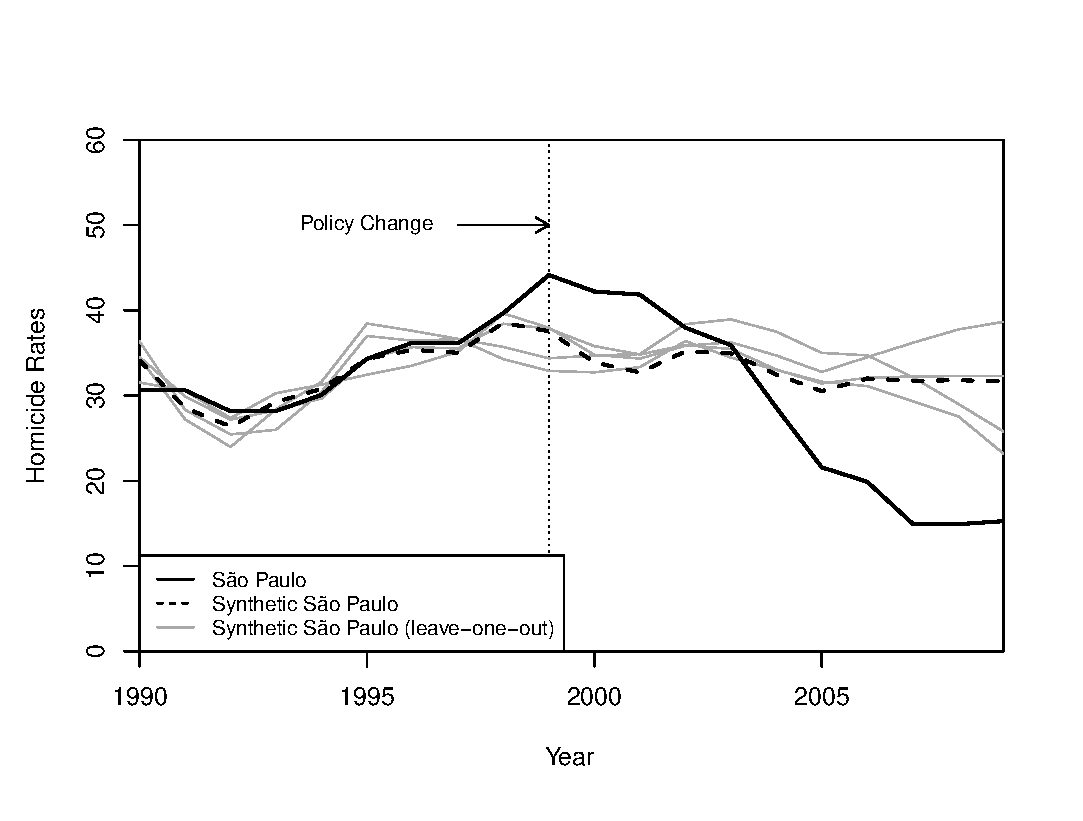
\includegraphics[width=.6\textwidth]{leave-one-out.eps}}
\caption{Leave-One-Out Distribution of the Synthetic Control for S\~{a}o Paulo.}\label{leave}
\end{center}
\end{figure*}

\section{Discussion}

As we have demonstrated, when compared to a synthetic control case, homicide rates were drastically reduced in S\~{a}o Paulo. Although it is not possible for us to estimate the treatment effect of each specific policy implemented during the 1990s and 2000s, we suggest that their aggregate impact was surely not negligible. In this regard, the state of S\~{a}o Paulo offers a clear example that it is feasible to fight crime with targeted policies. We see this as an encouraging result, as it suggests that governments can make progress in reducing crime with resources they already have at hand and need not rely exclusively upon structural conditions that are largely beyond their control such as unemployment, per capita income and inequality. Robustness tests provide further evidence for our findings.

Whereas the overall effects of the new security policies in S\~{a}o Paulo have been positive, it has also created adverse outcomes. Paradoxically, the recent increase in the prison population in the state of S\~{a}o Paulo---a by-product of harsher criminal policies---has created what today constitutes the most serious threat to public security in the state: the \textit{Primeiro Comando da Capital} (``First Command of the Capital'', PCC), Brazil's most powerful prison gang \citep{dias2009, souza2007}. The PCC staged two high-profile attacks against police forces (2001 and 2006), currently dominates about 90\% of the prisons in S\~{a}o Paulo, has established itself in 22 of the 27 Brazilian states, makes profits of about 50 million dollars per year, and has allegedly elected their own representatives in Brazil's last elections \citep{biondi2010}. Therefore, the state government now faces a considerable threat considering the increasing power and organization skills that the PCC currently possesses \citep{freire2014}.

Nonetheless, it could be that the reduction in homicide rates observed in S\~{a}o Paulo is due to more than one causal chain. Intuitively, one might think that because of better policing, there is an increased probability of a criminal getting caught, and so we should expect a decrease in crime rates given that the expected value of a crime is lower. However, another possibility to account for part of the effect observed in our study is the very empowerment of the PCC itself. If a sizeable number of homicides are drug-related and gang-related---specifically due to gangs competing for turf---then a reduction in homicide rates can be expected when we observe a monopoly in drug trafficking. This alternative causal mechanism works as follows: because of more efficient policing, the incarceration expectation of one who commits a crime is higher; because the criminal has a greater expectation of going to prison, he joins the PCC (either prior to or after being incarcerated), so he is more secure (either inside or outside prison); and finally, because the PCC has a stronger unity, it achieves a monopoly in drug dealing outside prison, resulting in less turf disputes, and consequently, less homicides \citep{skarbek2011}.

We also argue in favour of the Synthetic Control Method as a tool to evaluate government policies. This approach offers an intuitive way to assess causality claims when there is only a single treated unit, and it can be easily applied in a great number of situations. Given that there is a reasonable number of potential cases in the ``donor pool'', a synthetic control can be meaningfully compared to the actual case. In this way, the technique allows the researcher to use the potential outcomes framework even in unusual conditions. 

Future research can extend our findings in a number of ways. First, it would be interesting to test whether other criminal activities have been affected by the state government policies we mentioned previously. Since property crimes are pervasive in S\~{a}o Paulo, scholars could evaluate the causal link (or lack thereof) between public policies and the incidence of theft or robberies. Unfortunately, several states in Brazil do not publish time-series data for property crime, so we could not use the Synthetic Control Method for that dependent variable. As more data become available, this seems to be a good topic for scholars. Also, micro-level studies are needed to clarify the mechanisms behind S\~{a}o Paulo's homicide reduction. Due to the shortage of data on targeted policies, qualitative research may explain what the motivations, successes and shortcomings of S\~{a}o Paulo's recent security measures were. Further research could provide insights into how public policies work and, hopefully, help public authorities to design more effective policies against crime.

\newpage
\bibliographystyle{apalike2}
\bibliography{intelligent-policing}
\end{document}
